\subsection{Traduction automatique à base de transformeurs}
\label{sec. nmt-attention}

Le transformeur (ou modèle auto-attentif) est un modèle de séquence proposé en 2017~\cite{attention}.
Il vise à remédier aux lacunes des autres architectures utilisées en modélisation de séquences, 
notamment celles basées sur les \glsxtrshortpl{rnn} et les \glsxtrshortpl{cnn}.

En effet, les \glsxtrshortpl{rnn} souffrent de deux problèmes fondamentaux. 
Le premier est celui du mémoire à court terme, 
c--à--d, la tendance à négliger les dépendances entre unités lexicales éloignés dans la séquence.
Des variantes comme les \glsxtrshortpl{lstm} et surtout les \glsxtrshortpl{gru} 
ont réussi à éliminer ce problème au prix d'une augmentation dans la complexité des calculs.
Cependant, ces variantes, ainsi que les \Glsxtrshortpl{rnn} eux-mêmes, souffrent d'un deuxième défaut,
celui du calcul séquentiel.
Par conséquent, il n'est pas possible de paralléliser leurs calculs, 
ce qui les rends très lents~\cite{attention,deep-nmt-survey}.

Les \Glsxtrshortpl{cnn} permet de contourner les inconvénients posés par les \Glsxtrshortpl{rnn}.
Ils sont entièrement parallélisables, ce qui les rends extrêmement rapides à dérouler sur GPU.
De plus, ils peuvent calculer la dépendance entre deux positions arbitrairement éloignées.
Or, le nombre d'opérations qu'ils utilisent pour ce faire 
augmente avec la distance entre les deux positions en question.
De ce fait, ils sont également inadéquats pour la modélisation des corrélations à grande échelle~\cite{deep-nmt-survey}.

Le transformeur est une architecture à base à base de mécanisme d'attention 
qui offre une solution aux défis rencontrés par les autres architectures que nous avons introduites.
Il ne souffre pas du mémoire à court terme 
et peut calculer les dépendances globales de la séquence en temps constant~\cite{attention}.
La Figure~\ref{fig. transformer} illustre l'architecture d'un transformeur.
Il s'agit d'une architecture encodeur--décodeur.

\begin{figure}
    \begin{center}
        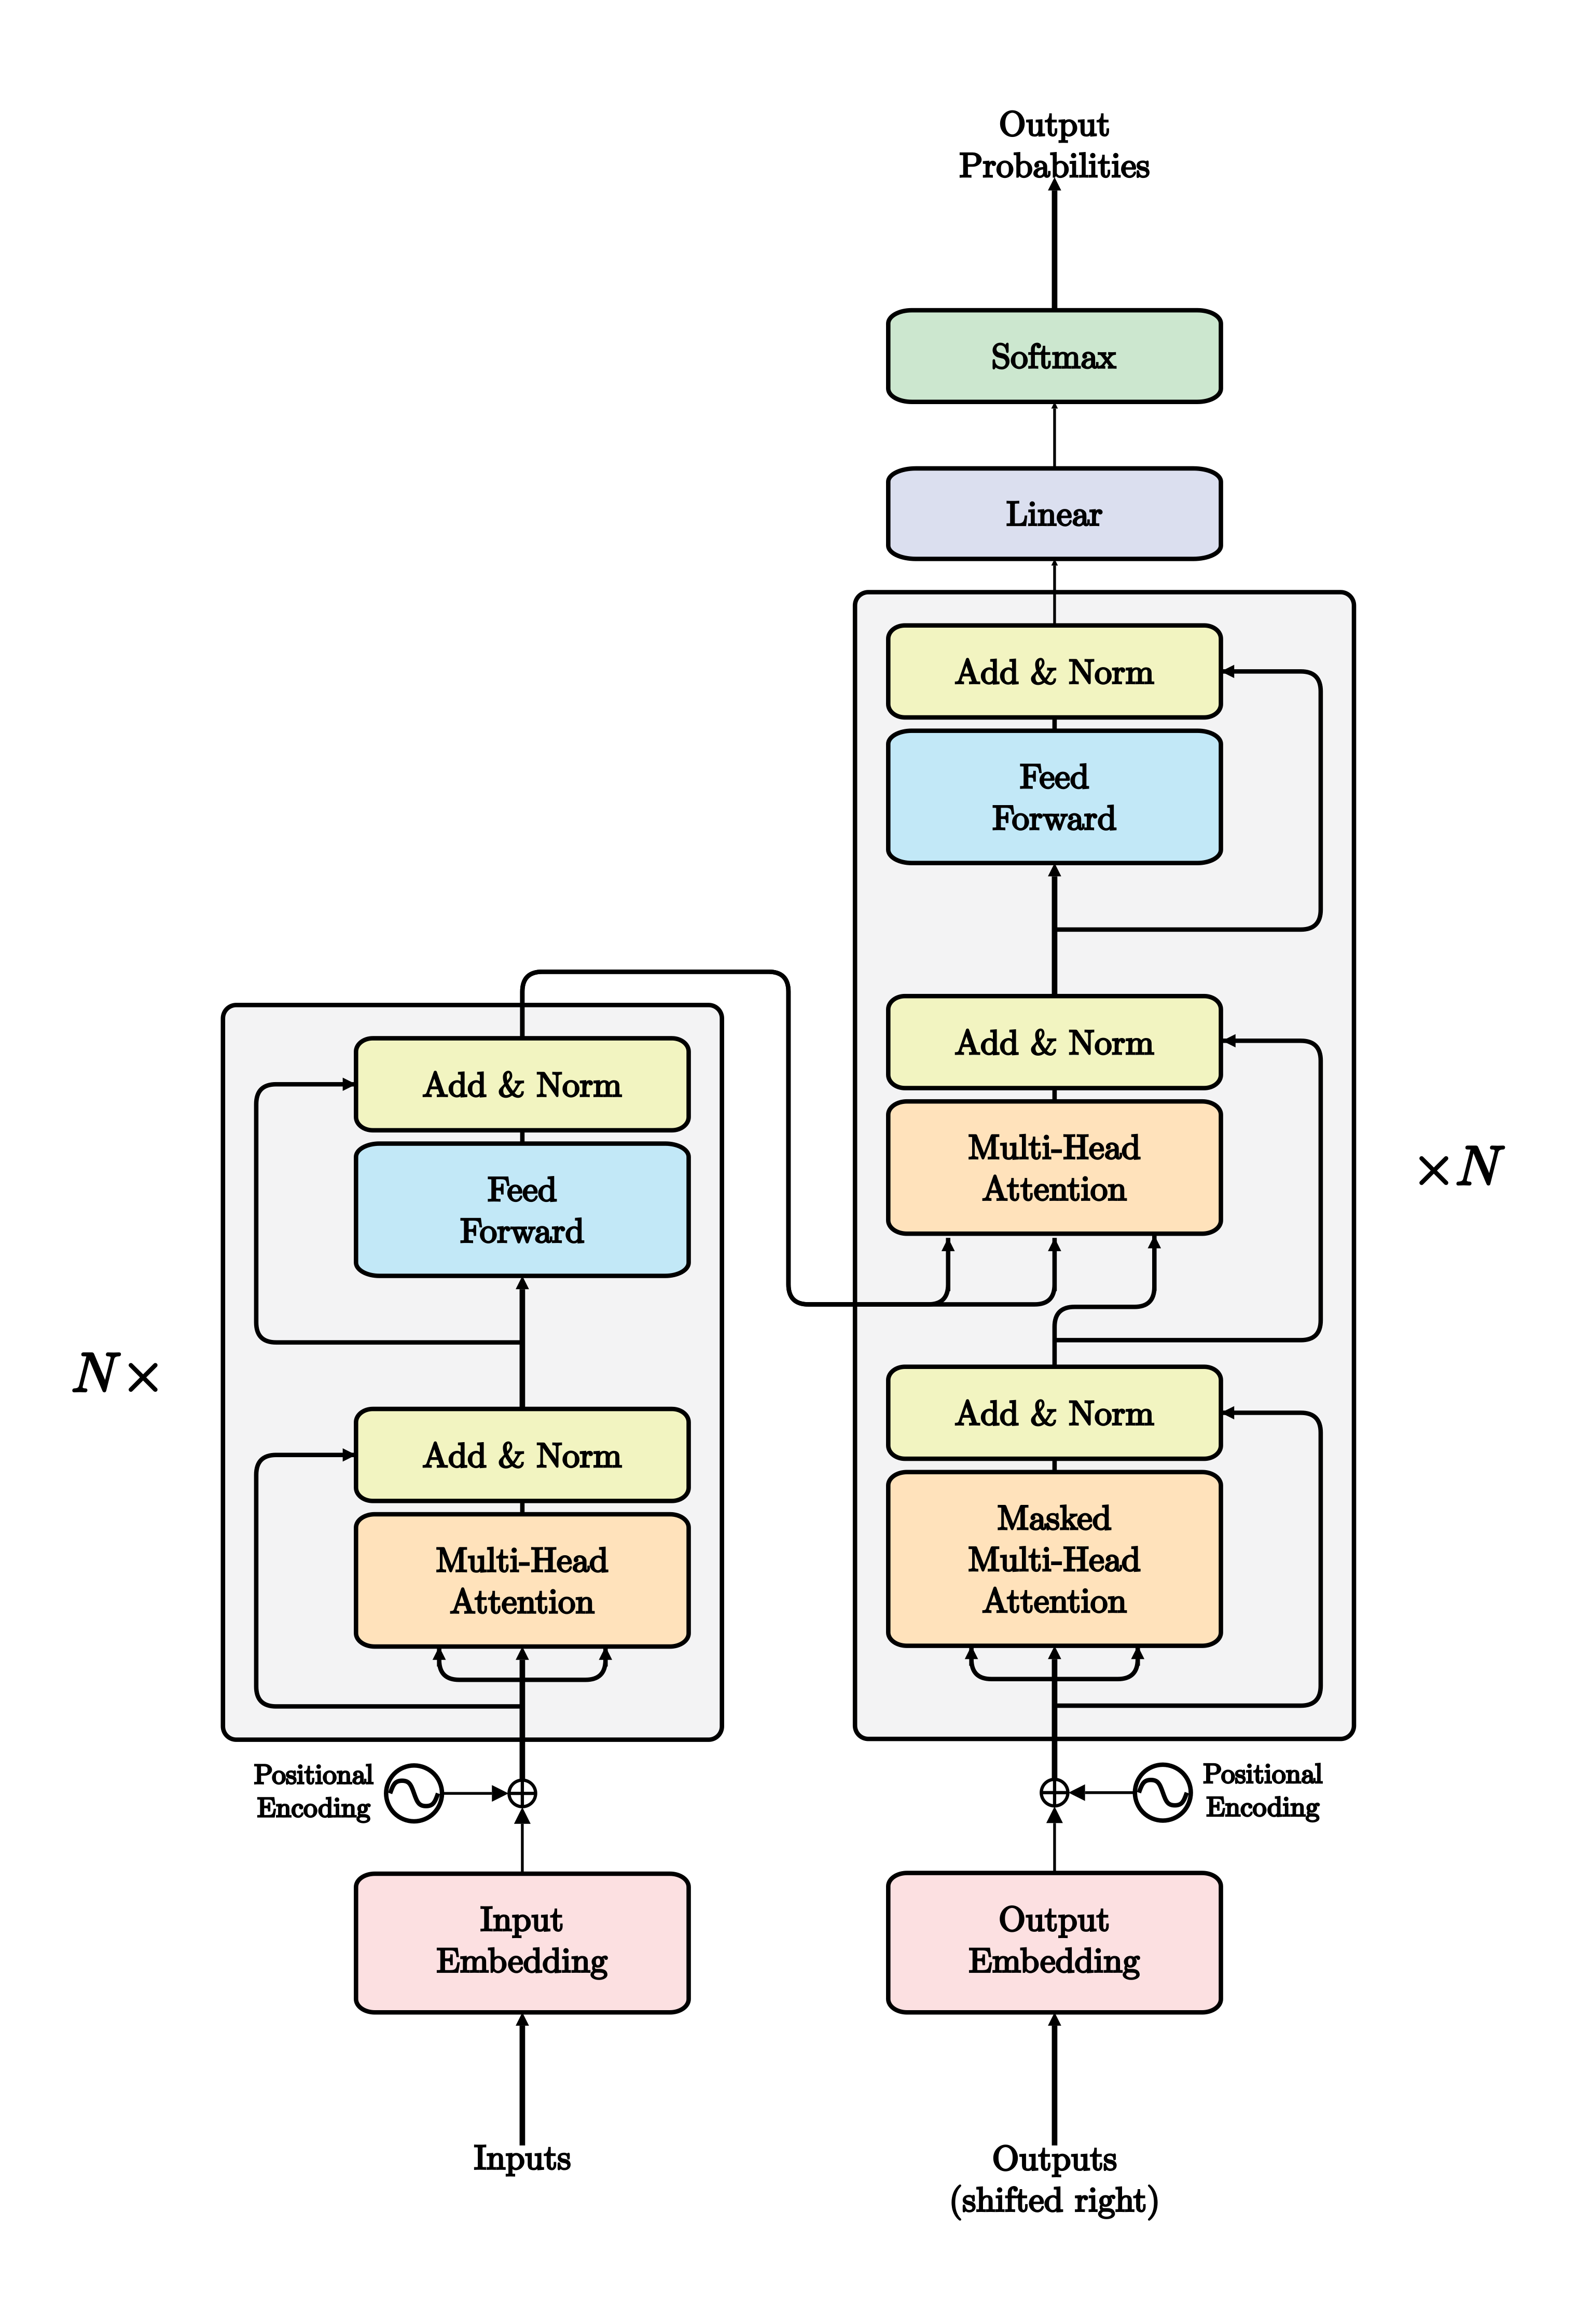
\includegraphics[width=10cm]{assets/images/transformer.png}
    \end{center}
    \caption[L'architecture du transformeur]
    {L'architecture du transformeur~\cite[Fig 1]{attention}}
    \label{fig. transformer}
\end{figure}

L'encodeur prend une séquence \((x_1, x_2, \cdots, x_n)\) de plongement de mots dans la \Glsxtrshort{ls} 
et produit une suite \((z_1, z_2, \cdots, z_n)\) de représentations vectorielles (vecteurs de pensée).
Cela est fait par le biais de l'Algorithme~\ref{algo. trans-encode} ou.

\[
    \operatorname{Attention}(Q, K, V)=\operatorname{softmax}\left(\frac{Q K^T}{\sqrt{d_k}}\right) V
\]
    
    

% \RestyleAlgo{ruled}
\begin{algorithm}
    \caption{Encoder une séquence}
    % \label{algo:trans-encode}
    \SetKwFunction{mha}{multi\_headed\_attention}
    % \DontPrintSemicolon
    \(x = (x_1, x_2, \cdots, x_n)\in\reals^n\) \comment{Plongement de la phrase d'entrée.}
    \(N\) \comment{Nombre d'itérations de l'encodeur.}
    \Deb{
        \(z \gets x\)
        \Pour{\(i = 1\cdots N\)}{
            \(z \gets \mha{z} + z\)
        }
    }
    \KwOut{\(z\in\reals^{n\times d}\) \comment{Thought vectors}}
\end{algorithm}

Le décodeur prend cette suite de représentations est produit une troisième séquence 
\((y_1, y_2, \cdots, y_n)\)
de mots dans \glsxtrshort{lc}.
